\section{System Detailed Design}
\label{sec:details}

In this section, we first present the overview of MicroPrivacy, then describe the details of each key component.

Figure~\ref{fig:architecture} shows the proposed MicroPrivacy framework.
In  Layer 1,  six modules are used: smartphone tilt angle, camera view angle, and angle of potential eavesdroppers, motion detection, face detection, and body detection.
We assume that three types of sensors are embedded into smartphones to act as input data for Layer 1, i.e, accelerator and gyroscope are used to estimate smartphone tilt angle, and camera sensor is used to capture image frames.
These modules provide input data for Layer 2.
In Layer 2, there are three key components:  (1) \textit{Privacy area Estimation} determines the area where potential visual eavesdropping may occur. (2) \textit{Visual detection inside the camera view} combines face detection and motion detection  to detect human visible by the camera. (3) \textit{Prediction outside the camera view} predicts the probability of visual eavesdroppers based on the estimated movement speed and direction of the eavesdropper while he's inside the camera monitoring area.
In Layer 3,  the visual eavesdropper detection algorithm determines whether to alert the user or not.

\begin{figure}[H]\label{framework}
\centering
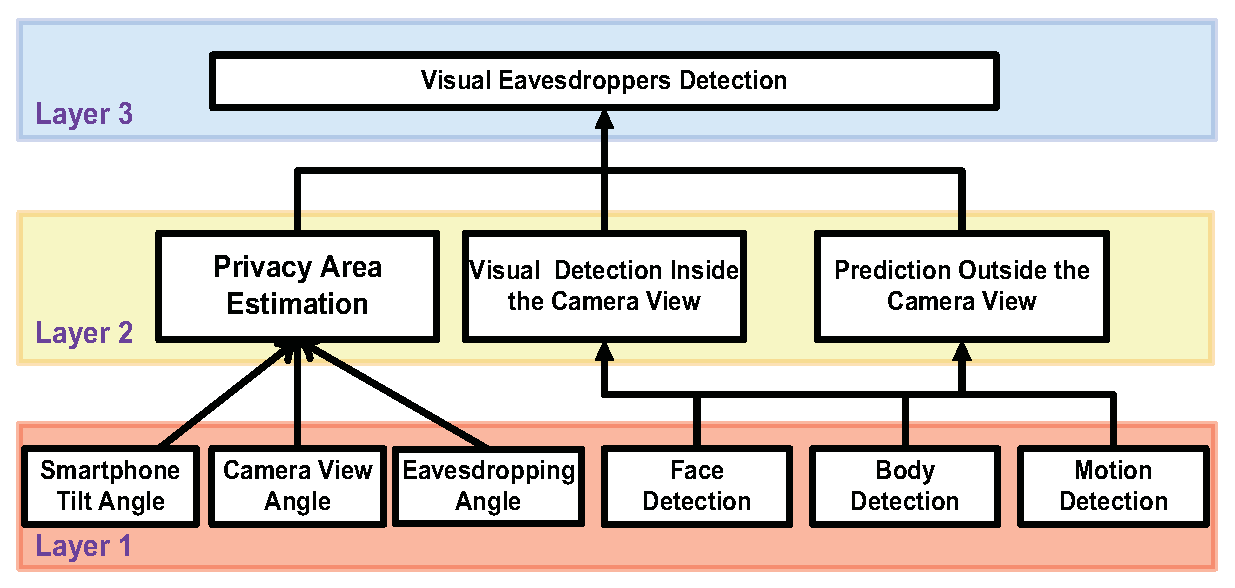
\includegraphics[width=3.5in]{framework.eps}
\caption{Architecture of  visual eavesdroppers detection}
\label{fig:architecture}
\end{figure}

\subsection{Privacy Area Estimation}

The size of the privacy area determines the scope the front camera is able  to cover.
First, we  define four types of areas to represent the situation that the visual eavesdropper detection algorithm works differently.
We then derive a formula to estimate the size of the privacy area taking into account  the visual distance, and the phone tilt angle, and the area blocked by user.

\subsubsection{Definition of the Privacy Area}
As Fig.~\ref{fig:area} shows, the red area (i.e., the monitoring area) represents the front camera field of view and the blue area (i.e., the privacy impaired area) shows the range that the visual eavesdroppers can see the information on smartphone screen. The overlap of the two areas is denoted as $A_{11}$, the part of the impaired area that is out of the monitoring area is denoted as  $A_{10}$,  the part of the monitoring area that falls out of the privacy impaired area is denoted as $A_{01}$,  and the area that is outside both monitoring and privacy impaired areas is $A_{00}$. Typically, $A_{01}$ is  very small  and $A_{00}$ is the unconcerned area. We further use $\alpha_h$, $\alpha_v$ to represent the horizontal and vertical angle of the camera view respectively. The angle of potential eavesdropping is defined as $\beta$. Therefore, at  distance $d$, the monitoring area  (i.e., $(A_{11}+A_{01})_d$) can be expressed as $d^2\tan^2\beta$ and the privacy impaired area  (i.e., $(A_{11}+A_{10})_d$) is $d^2\tan\alpha_v\tan\alpha_h$.
\begin{figure}[H]
\centering
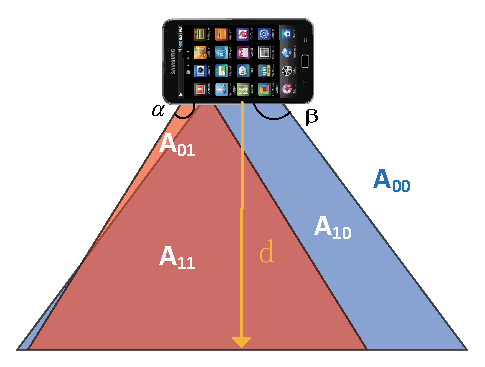
\includegraphics[width=2in]{area1.eps}
\caption{Definition of different areas }
\label{fig:area}
\end{figure}


\subsubsection{Issues for Determining Area Size}


The size of privacy impaired area is affected by three factors:  visual distance $d$,  phone  tilt angle $\theta$, and size of the area blocked by user.

\textbf{Visual distance.} To estimate the privacy area, we should measure the maximum visual distance that a person can see the text on smartphone (Fig.~\ref{fig:distance}). In our daily life, we use the eye chart to measure the visual acuity (i.e., how far  a person can see clearly). We determine the visual distance by considering the phone screen as an eye chart with the international definition of visual acuity \cite{acuity}.  The visual distance is expressed as:
\begin{equation}
\begin{split}
& d=\frac{acuity*font size}{gap size*tan\theta^*}
\end{split}
\end{equation}
where $\theta^*=0.0167$ is a visual angle of 5 arc minutes and $gapsize$ is 5 based on the design of a typical optotype. \textit{Acuity} is the value used in the international definition of visual acuity and we set acuity value to 20/20=1.0, the standard visual range of the human.  \textit{fontsize} represents the height of the font on the phone screen. The screen size of the smartphone  ranges from 3 inches to 6 inches and font size is no larger than 10.7 mm. This gives the maximum visual distance of 5 meters.
\begin{figure}[H]
\centering
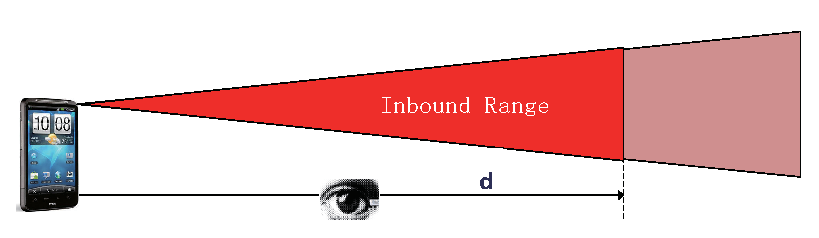
\includegraphics[width=3.5in]{distance.eps}
\caption{Estimation of  visual distance}
\label{fig:distance}
\end{figure}


\textbf{Tilt angle of the phone.}
The phone rotation affects the area size (Fig.~\ref{fig:rotation}).  With the angle of the phone rotation $\theta$ and distance $d$, the monitoring area is  $d^2\tan^2\beta\tan\theta$ and  privacy impaired area is $d^2\tan\alpha_w\tan\alpha_h\tan\theta$.
\begin{figure}[H]
\centering
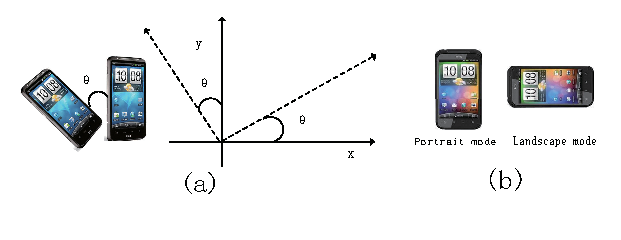
\includegraphics[width=3.5in]{rotation.eps}
\caption{(a) The angle of the phone rotation (b) The camera view mode}
\label{fig:rotation}
\end{figure}

\textbf{Size of user-blocked area.}
When the camera view of the smartphone is blocked by the user's face, the blocked area has no use for face detection and affect the performance of the visual eavesdroppers, even though it is part of the monitoring area, so we need to determine the size of the blocked area (Fig.~\ref{fig:block}).
\begin{figure}[H]
\centering
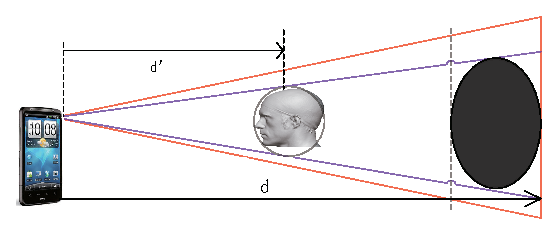
\includegraphics[width=3.5in]{blockedarea.eps}
\caption{The user's face blocks the camera view }
\label{fig:block}
\end{figure}

Assume that the face height in the camera is defined as $f_h$ and the camera focus is expressed as $fos$ (available through Android API), we can derive the distance $d'$ between face and camera by using the pinhole camera model \cite{PinholeModel}. The pinhole camera model describes the mathematical relationship between the coordinates of a point and its projection onto the image plane of an ideal pinhole camera.
\begin{equation}
d'=\frac{fos*face\_height}{f_h}
\label{eqn:d'}
\end{equation}
where $face\_height$ is the actual face height in millimeters,
$f_h=\frac{f_h(p)*res_h}{s_h*dpi*0.3937}$, note that 1 cm $\approx$ 0.3937  inches.  $f_h(p)$ is the face height measured in pixels on smartphone, dpi is dots per inch, $res_h$ is screen height resolution  and  $s_h$ is image height size.  They can all be obtained via Android APIs.
%The face height $f_h$ can be calculated by the face height . Android APs can provide the dpi (dots per inch), screen height resolution $res_h$ and image height size $s_h$, so we can compute face height in camera $f_h=\frac{f_h(p)*res_h}{s_h*dpi*0.3937}$  (1 cm $\approx$ 0.3937  inches.).
The range of the face size is limited and the  estimation of the face size is difficult. Therefore, we set the face height to the average size of 220mm instead of estimating one's actual face height. Therefore, we can use Eq.~\ref{eqn:d'} to calculate the distance $d'$ between camera and face. %For estimating the blocked area at distance $d$, we need to know the face height $f_h$ and width $f_w$ in camera.
The aspect ratio of face width and height in an image is the same as in reality, so with the face width measured in pixels available via Android API, we can compute $f_w$ in a similar way as computing $f_h$.  Therefore,
\begin{equation}
\textrm{size of blocked area} = f_w*f_h\frac{d}{d'}
\end{equation}


\subsubsection{Computation of Privacy Area Size }
To calculate size of the monitoring and privacy impaired area, we use the tilt angle of the phone ($\theta$), camera view angle ($\alpha_v$ and $\alpha_h$), and the  angle of a potential visual eavesdropper ($\beta$). In addition, we take into account the area blocked by the phone user, which is determined by  face height ($f_h$), face width ($f_w$), and distance ($d'$).
Based on the discussions previously, we have the  size of the monitoring area and privacy impaired area at distance $d$ as follows.
\begin{equation}
\begin{split}
& (A_{11}+A_{01})_d=d^2\tan^2\beta\tan\theta-f_w*f_h\frac{d}{d'}\\ %\textrm{size of monitoring area} =
& (A_{11}+A_{10})_d=d^2\tan\alpha_w\tan\alpha_h\tan\theta-f_w*f_h\frac{d}{d'} %\textrm{size of privacy impaired area} =
\end{split}
\end{equation}


\subsection{Detection inside the camera view}
When an eavesdropper stays inside the camera view, we use a visual detection algorithm to discover him.
Given two image frames, visual human detection  aims to detect human in the monitoring area by combining face detection and body detection.

%\subsubsection{Face Detection}
Face detection can help detect human and plays a important role in detecting the visual eavesdropper. Many face detection methods have been proposed \cite{viola2004robust} and shown their effective using public datasets. The face detection APIs or libraries are available from opencv\cite{opencvFace}, android\cite{androidFaceAPI}, and other open source projects\cite{MicrosoftFace}. In MicroPrivacy, we integrate different APIs to run our system on different platforms. The basic face detection algorithm is based on the Haar cascade algorithm \cite{viola2004robust}.

%\subsubsection{Body Detection} \label{dt:motion}
Many computer vision algorithms have been designed to track and detect objects such as human body\cite{felzenszwalb2008discriminatively}\cite{wang2009hog}.  However, we adopt a motion detection method to track the body. Even with limited  computation power of mobile phones, motion detection  is still fast and effective for  camera-based apps. As Fig.~\ref{fig:motion} shows, the proposed method uses two frames to get the object and considers the center of the object as the key point for tracking.  Specifically, we use frame difference method \cite{lee2009vision} that subtracts two frame for detecting the moving object. The centroid of the moving object is considered as a key point.  %Compared with using two key points from three frames, we can easily get the motion direction and  speed. Further,
 Motion detection  can generate human trajectories  that can be very handy for potential eavesdropping even when the person is invisible in the camera.
\begin{figure}[H]
\centering
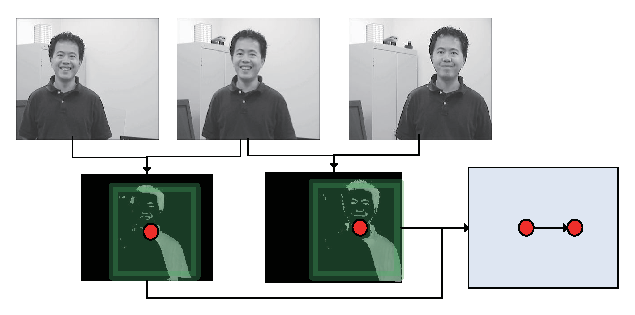
\includegraphics[width=3.5in]{motion.eps}
\caption{Motion detection using the Mhyang tracking database}
\label{fig:motion}
\end{figure}


%\subsubsection{Fast detection}
 We propose to speed up the visual detection algorithm.  Intuitively, we reduce the size of privacy area which reduces the computation of visual detection algorithm. We first remove the user-blocked area from the monitoring area of the front camera.
Usually, the smartphone user face takes a large space in the image size. Removing it will speed up  visual detection algorithm.
We then process the frames with the face-blocked area removed. In this way,  face detection can be significantly accelerated. Fig.~\ref{fig:remove} is an example of this process using the Caltech dataset~\cite{jesorsky2001robust}.
The left is the original image that consumes more computation than the right  with the face removed from the image.
\begin{figure}[H]
\centering
\includegraphics[width=3.5in]{face.eps}
\caption{Remove the blocked area for fast face detection (the original image is from the Caltech dataset)}
\label{fig:remove}
\end{figure}

%Remove the blocked area for fast face detection every few seconds from the monitoring area, we only need to detect faces in the other part.   the Face detection method can be speed up by removing the blocked area caused by the occlusion of the phone user's face. If we remove the blocked area from the monitoring area, we only need to detect faces in the other part.  %We propose a polling mechanism to implement this method. This polling mechanism locate the position of the user's face and remove it every time, just as a timer.  Specifically, We use face detection to detect the full image and remove the largest face area every few seconds. During this interval,




\subsection{Prediction outside the camera view}
A visual eavesdropper may move out of the camera's monitoring area but can still see  the phone's screen.
% if the viewer is initially in that area, then this approach will not work.
To detect this,  we estimate the probability of this situation. The basic idea  is to use the historical human trajectory to predict its next  location. If the predicted location is still in the privacy impaired area, the invisible eavesdropper is considered to be detected.

We use maximum likelihood estimation to build a probability model for this detection:
\begin{equation}
\begin{split}
& P(t,\tau|M)=P(t|M)P(\tau|M),
\end{split}
\end{equation}
where $t$ is the duration of the detected face that disappears from the monitoring area and $\tau$ is the duration of the detected  body that disappears from the monitoring area. $M$ is the parameter to be be estimated for maximizing the likelihood probability $P(M|t,\tau)$. Three aspects of the parameter $M$ can be used for determining the data distribution and they are direction, speed, and area size. %and expressed as $M=\{direction,speed,area size\}$.
We use these three elements to build a probability model to determine $M$.  Instead of obtaining $M$ from training data as a typical maximum likelihood estimation method, we get it from the human detection model;  the goal is the same, i.e., to maximize the likelihood probability $P(M|t,\tau)$.  Specifically, we use face detection and motion detection  to record the human's trajectory. Once the detected human  disappears from the camera view, we calculate the motion direction and speed from the records, predict the possible location of the human. We use the area size  to estimate the possible time duration that the invisible person can still  read the phone screen. The probability of the invisible person eavesdropping is expressed as follows (Fig.~\ref{fig:invisible}).
\begin{equation}
P(t|M)=P(\tau|M)=1-\frac{v*t}{d^*\cos\gamma(\tan\beta-\tan\alpha)+\epsilon}
\label{eqn:prob}
\end{equation}
where $v$ is the motion speed, $\gamma$ is the motion direction,  $d^*$ is the distance between object's face and camera, and  $\epsilon$ is a smoothing factor to avoid the exception of division by zero. $\alpha$ is set to $\alpha_v$ or $\alpha_h$ while the phone is in vertical ro horizontal.
%that is mentioned in \textit{Area Estimation} section.
\begin{figure}[H]
\centering
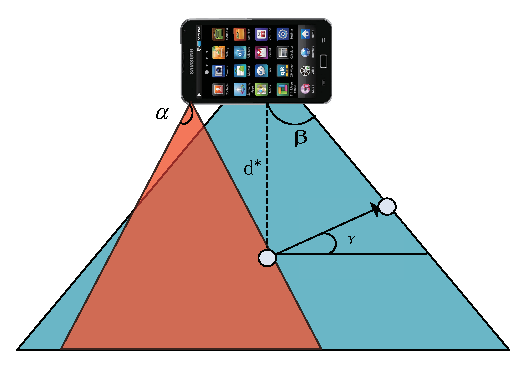
\includegraphics[width=2.5in]{areaMotion.eps}
\caption{Prediction of eavesdropper outside camera view}
\label{fig:invisible}
\end{figure}



There is another situation for predicting the location of the visual eavesdropper, i.e., the visual eavesdropper  moves into the user blocked area. This area is inside the monitoring view but is blocked by phone user's face (Fig.~\ref{fig:invisible-blocked}).
\begin{figure}[H]
\centering
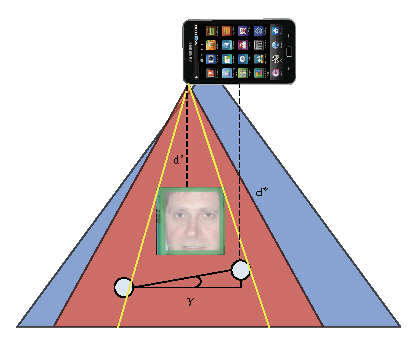
\includegraphics[width=2.5in]{areaMotionBlocked.eps}
\caption{ Human prediction in area blocked by user face}
\label{fig:invisible-blocked}
\end{figure}
In this case, the probability of the invisible human eavesdropping is expressed as:
\begin{equation}
P(t|M)=P(\tau|M)=1-\frac{v*t}{d^*\cos\gamma*(f_w*\frac{d^*}{d'})+\epsilon}
\label{eqn:prob}
\end{equation}


%The method discussed previously uses
%The two thresholds $t$ and $\tau$ used in the method discussed previously should be adaptive to the environment in terms of noise level, crowded or not, or whether many people are passing by, etc.  We propose a methodology for threshold selection (Fig.~\ref{fig:env}).   It consists of three steps.  (1) \textit{Multi-sensor Fusion} collect data from WiFi, GPS, and acoustic sensor to generate fused data.(2) \textit{Environment Perception} uses support vector machine  to classify the environment. (3) \textit{Threshold Learning} uses AdaBoost~\cite{} to learn the proper thresholds.
%\begin{figure}[H]
%\centering
%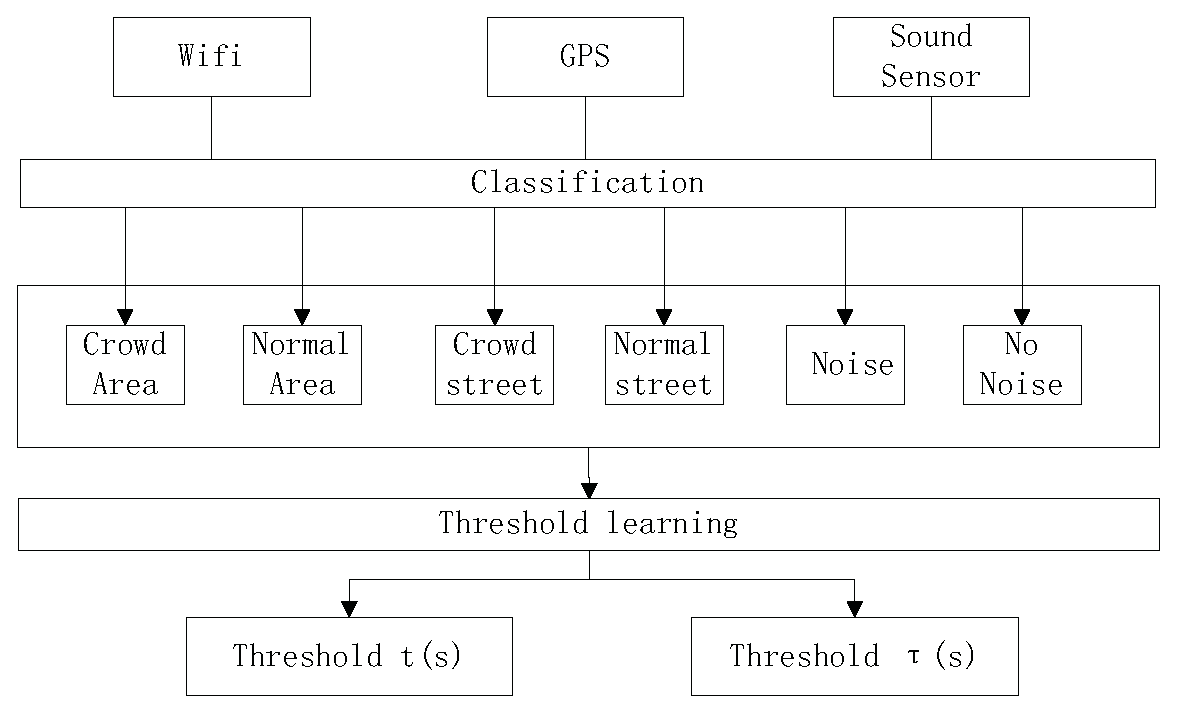
\includegraphics[width=3.5in]{sensorfusion.eps}
%\caption{The architecture of environment perception with sensor fusion.  }
%\label{fig:env}
%\end{figure}

\subsection{Visual Eavesdropper Detection Algorithm}
A visual eavesdropper is a person who stays around the user and watches the user's phone screen for a time duration longer than the threshold.  Since  we use face detection and motion detection to detect human, it is necessary to record the face detection time $t_h$ and the motion detection time $\tau_f$. If we denote   $f(\tau_f,\textit{t}_h)$ as the visual eavesdropper detection result, then
\begin{equation}
f(\tau_f,\textit{t}_h)=
\begin{cases}
1 & \text{if}\,\tau_f>\tau(s) \textrm{ or } \textit{t}_h>\textit{t}(s)\\
0 & \text{otherwise}
\end{cases}
\end{equation}
where $t_h$ represents the time of the human body in the privacy impaired area,  $\tau_f$ represents the time that the person looks at the phone screen, $\tau(s)$ and $t(s)$ are the thresholds to indicate time duration that a normal person stays.
A person is considered as a visual eavesdropper if detected face time $\tau_f$ is larger than the threshold $\tau(s)$ or detected body time $\textit{t}_h$  is larger than the threshold \textit{t}(s).
The threshold is sensitive to the environments around the smartphone user. For instance, the time threshold on the bus station should be different from the classroom.  According to the experience or the feedbacks of smartphone users, we set the time threshold $\tau(s)$ and \textit{t}(s) to empirical values.



%Putting it all together, the entire algorithm is shown in Algorithm~\ref{alg:Framework}.
Algorithm~\ref{alg:Framework} describes the overall algorithm of our visual eavesdropper detection.
We first calculate the privacy area using Eq. (4) based on camera angles ($\alpha_v,\alpha_h$), title angle of the phone ($\theta$), and visual distance ($d$) (Line~\ref{alg:line:1}).  If the front camera detectes the face of a visual eavesdropper, we add one to the time variable $\tau_f$ that represents the storage time of face detection (Line~\ref{alg:line:2}).  If the body of the eavesdropper is detected by front camera, the time variable $\tau_h$ needs to increment by one, which denotes the storage time of body detection  (Line~\ref{alg:line:3}).
%We directly added the unit time to the time variable, if  eavesdroppers are fall within the side of camera coverage.
When an eavesdropper falls outside the camera view, we use Eq.(~\ref{eqn:prob}) to calculate the time  variables $\tau_h$ and  $\tau_f$ (Line~\ref{alg:line:4})..
Finally our algorithm determines whether there is a   visual eavesdropper or not (Line~\ref{alg:line:5}).

\begin{algorithm}[H]
\caption{Visual Eavesdroppers Detection}
\label{alg:Framework}
\begin{algorithmic}[1]
\REQUIRE  face detection $t(s)$, body detection  threshold $\tau(s)$ , camera angles ($\alpha_v,\alpha_h$), title angle of the phone ($\theta$), visual distance ($d$)
\ENSURE   Visual eavesdropper detection result;
             alerts to user;
\STATE Calculate privacy area using Eq.(4);
\label{alg:line:1}
\STATE Connect to the front camera initially;
\STATE Initialize  face detection time $\tau_f=0$;
\STATE Initialize body detection time $\textit{t}_h=0$;
\REPEAT
\STATE Get the current frame from the front camera;
%\STATE Processing the received frame;
\STATE Run face detection algorithm;
\STATE Run human motion detection algorithm;
\IF  {\textit{detected  human in previous frame} }
\STATE Calculate motion direction $\gamma$ and motion speed $v$
\ENDIF
\IF  {\textit{detected  human face}}
\STATE $\tau_f=\tau_f+1$; Calculate  total face detection time
\label{alg:line:2}
\ENDIF

\IF  {\textit{tracked  motion of  human body}}
\STATE $\textit{t}_h=\textit{t}_h+1$;  Calculate  total motion detection time
\label{alg:line:3}
\ENDIF
\IF  {\textit{face detection failed} and \textit{motion detection failed}}
\STATE Estimate $R_h$ and $R_f$ based on Eq.~\ref{eqn:prob}:
\STATE $\textit{t}_h=\textit{t}_h+P(t|M)$;
\STATE $\tau_f=\tau_f+P(t|M)$;
\label{alg:line:4}
\ENDIF
\IF  {\textit{$t_h$}$\geq$\textit{t}(s) or  $\tau_f \geq\tau(s)$ }
\label{alg:line:5}
\STATE Label the human as a visual eavesdropper;
\STATE $f(\tau_f,\textit{t}_h)=1$;
\STATE $\tau_f=0$ and $\textit{t}_h=0$;
\STATE Alert the user about the  privacy leakage;
\ENDIF
\UNTIL User terminates the application




\end{algorithmic}
\end{algorithm}


